%
% LaTeX-Rahmen f�r Arbeiten am Lehrstuhl Hegering
%
% Harald Roelle, 2001, 2002
% Modified by Nils gentschen Felde, 2006
%
% basierend auf Arbeiten von Helmut Reiser, Boris Gruschke und Stephen Heilbronner
%


%Link im PDF
\ifpdf
  \pdfbookmark[0]{Titel}{Titel}%
\fi

%%%%%%%%%%%%%%%%%%%%%%%%%%%%%%%
% erste Seite

\thispagestyle{empty}

\begin{center}


\includegraphics[width=3cm]{tum-logo}

\vspace{1cm}

{\Huge FAKULT�T F�R INFORMATIK\\[1mm]}
DER TECHNISCHEN UNIVERSIT�T M�NCHEN\\

\vspace{2cm}

{\Large \textbf{\typeOfThesis\ in Informatik}}\\

\vspace{2.0cm}
{\Huge \textbf{\titleOfThesisOne}}\\
\vspace*{3mm}
{\Huge \textbf{\titleOfThesisTwo}}\\
\vspace*{3mm}
{\Huge \textbf{\titleOfThesisThree}}\\

\vspace{1.5cm}

\parbox{1cm}{
  \begin{Large}
    \begin{tabbing}
%      Bearbeiter: \hspace{5mm}
        \authorOfThesis\\[2mm]
%      Aufgabensteller:
%        \>\aufgabensteller\\[2mm]
%      Betreuer: 
%        \>\betreuerOne\\
%        \>\betreuerTwo\\[2mm]
%        \>\betreuerThree\\
%      Abgabetermin: 
%        \> \abgabeTagZahl.~\abgabeMonatText~\abgabeJahrZahl\\
    \end{tabbing}
  \end{Large}
}\\

\vspace{10mm}

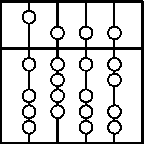
\includegraphics[width=2.4cm]{tum-abakus}

\end{center}

\newpage

%%%%%%%%%%%%%%%%%%%%%%%%%%%%%%%
% zweite Seite

\thispagestyle{empty}
\cleardoublepage 

%%%%%%%%%%%%%%%%%%%%%%%%%%%%%%%
% dritte Seite

\thispagestyle{empty}

\begin{center}


\includegraphics[width=3cm]{tum-logo}

\vspace{1cm}

{\Huge FAKULT�T F�R INFORMATIK\\[1mm]}
DER TECHNISCHEN UNIVERSIT�T M�NCHEN\\

\vspace{2cm}

{\Large \textbf{\typeOfThesis\ in Informatik}}\\

\vspace{2.0cm}
{\Huge \textbf{\titleOfThesisOne}}\\
\vspace*{3mm}
{\Huge \textbf{\titleOfThesisTwo}}\\
\vspace*{3mm}
{\Huge \textbf{\titleOfThesisThree}}\\

\vspace{1.5cm}

\parbox{1cm}{
  \begin{large}
    \begin{tabbing}
      Bearbeiter: \hspace{1cm}
        \=\authorOfThesis\\[2mm]
      Aufgabensteller:
        \>\aufgabensteller\\[2mm]
      Betreuer: 
        \>\betreuerOne\\
        \>\betreuerTwo\\
      Abgabedatum: 
        \> \abgabeTagZahl.~\abgabeMonatText~\abgabeJahrZahl\\
    \end{tabbing}
  \end{large}
}\\

\vspace{5mm}

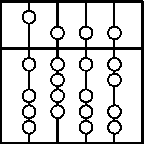
\includegraphics[width=2.4cm]{tum-abakus}

\end{center}
